\chapter{TINJAUAN PUSTAKA}
\label{chap:tinjauanpustaka}

% Ubah bagian-bagian berikut dengan isi dari tinjauan pustaka

\section{Hasil Penelitian Terdahulu}
\label{sec:hasilpenelitianterdahulu}

\subsection{Applying Generative Adversarial Networks to Intelligent Subsurface Imaging and Identification}
\label{sec:apllyingGANtoISII}

William Rice melakukan penelitian terkait penerapan metode GAN untuk mendeteksi objek bawah permukaan tanah. 
Dalam penelitiannya, objek yang dideteksi berupa silinder dengan 3 jenis bahan, yaitu besi, plastik, dan beton yang terkubur di bawah permukaan tanah. 
Penelitian ini menggunakan metode FDTD dalam modelnya. 
Hasil penelitian ini menunjukkan bahwa metode GAN dapat digunakan pada data GPR, baik dari data asli maupun data simulasi GPR. 
\emph{Class conditioning} dapat diterapkan pada metode GAN dalam menghasilkan \emph{training data} yang terlabel untuk klasifikasi.
Dengan \emph{training data} ini, terlihat bahwa augmentasi GAN dapat meningkatkan pengklasifikasi. \parencite{Rice2019ApplyingGA}.

\subsection{Early Detection of Near-Surface Void Defects in Concrete Pavement Using Drone Based Thermography and GPR Methods - Final Report}
\label{earlydetectionGPRmethod}

Zhigang Shen beserta tim melakukan penelitian dengan 2 metode berbeda dalam mendeteksi cavities pada beton yang masih baru dicetak, yaitu dengan pendekatan \emph{Infrared Thermographic} dan \emph{Ground Penetrating Radar} (GPR). 
Penelitian dengan pendekatan GPR bertujuan untuk mengetahui batasan penggunaan GPR pada beton pasca pengecoran. 
Untuk menghindari kerusakan pada beton pasca pengecoran, sebuah papan triplek digunakan sebagai penampang GPR agar tidak menyentuh beton secara langsung. 
Hasil penelitian menunjukkan bahwa GPR dapat menjadi metode \emph{non-destructive testing} (NDT) untuk mendeteksi \emph{cavities} dengan ukuran 3.8 cm hingga 10 cm pada saat 3 jam setelah pengecoran beton. \parencite{earlyDetectionofNearSurfaceVoidDefect}

\subsection{Image-to-Image Translation with Conditional Adversarial Networks}
\label{image2imagetranslationCGAN}
Philip Isola beserta timnya melakukan penelitian terkait penggunaan \emph{Conditional Adversial Networks} (cGAN) dalam mengubah dari suatu gambar ke gambar lain. 
Penelitian ini mendemonstrasikan penggunaan pix2pix dalam mensintesis foto dari bentuk label kasaran menjadi suatu gambar objek tertentu. 
Dari penelitian disimpulkan bahwa penggunaan cGAN sangat menjanjikan dalam permasalahan perubahan gambar satu ke gambar lain, terkhususnya yang membutuhkan output terstruktur. \parencite{image2imageCGAN}

\section{Cavities}
\label{sec:cavities}

\emph{Cavities} atau \emph{void}, merupakan suatu rongga kosong yang terbentuk pada beton akibat udara yang terperangkap di dalamnya. 
Ketika beton selesai dicor, sebagian besar udara yang terperangkap keluar dari campuran. 
Udara terperangkap yang tersisa dalam campuran kemudian menciptakan kekosongan udara pada beton. 
Cavities pada beton dapat ditimbulkan oleh berbagai sebab, diantaranya: Pemadatan yang dilakukan dengan vibrator kurang baik, 
karena jarak antar bekisting dengan tulangan atau jarak antar tulangan terlalu sempit sehingga bagian mortar tidak dapat mengisi rongga antara agregat kasar dengan baik. \parencite{analisakerusakanbeton}

\section{Ground Penetrating Radar}
\label{sec:groundPenetratingRadar}

\emph{Ground Penetrating Radar} (GPR) merupakan salah satu metode geofisika dalam mengidentifikasi kondisi bawah permukaan. 
Penggunaan GPR pada awalnya digunakan untuk bahan geologi pada alam. 
Seiring berkembangnya teknologi, GPR dapat diterapkan untuk media jenis lainnya, seperti kayu, beton, dan aspal \parencite{jol2008ground}.

\begin{figure}[ht]
  \centering
  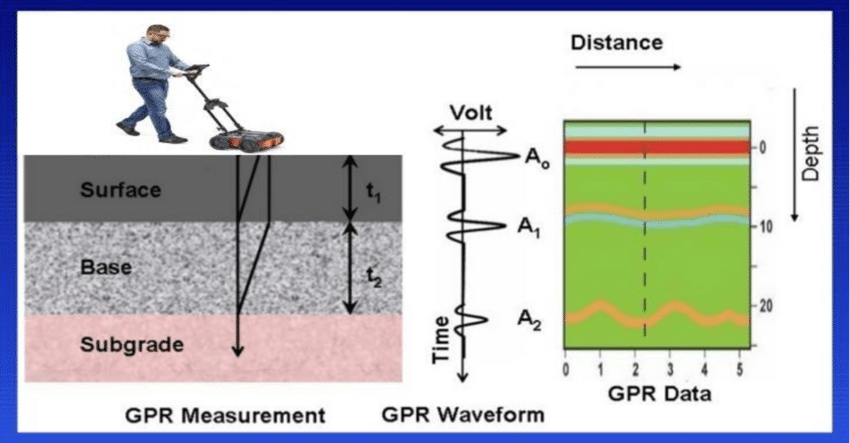
\includegraphics[scale=0.35]{gambar/prinsipGPR.png}
  \caption{Prinsip Kerja GPR Secara Umum \parencite{gprPrinciple}.}
  \label{fig:prinsipGpr}
\end{figure}

GPR terbagi menjadi 2 bagian, yaitu bagian antena pemancar (transmitter) dan bagian antena penerima (receiver). 
Garis besar sistem GPR dapat dilihat pada gambar \ref{fig:prinsipGpr}. 
Antena pemancar dan penerima biasanya identik dan memenuhi karakteristik bentuk gelombang yang dihasilkan. 
Antena pemancar membangkitkan sinyal listrik ke dalam tanah. 
Selama perambatan, sinyal akan mengalami berbagai kerugian (loss). 
Jika sinyal bertabrakan dengan bahan yang tidak homogen dengan media perambatan, maka sinyal akan dipantulkan. 
Sinyal ini akan diterima dan diproses oleh antena penerima.

\subsection{GprMax}
\label{subsec:gprMax}

GprMax merupakan open source software yang mensimulasikan propagasi gelombang elektromagnetik. 
GprMax memecahkan persamaan Maxwell dalam 3D menggunakan metode Finite-Difference Time-Domain (FDTD). 
GprMax dirancang untuk pemodelan Ground Penetrating Radar (GPR) tetapi juga dapat digunakan untuk memodelkan propagasi gelombang elektromagnetik untuk banyak aplikasi lainnya. 

\begin{figure}[ht]
  \centering
  
\includegraphics[scale=0.35]{gambar/gprMax.png}
  \caption{Logo gprMax (sumber : www.gprmax.com).}
  \label{fig:logogprMax}
\end{figure}

GprMax saat ini dirilis di bawah GNU General Public License v3 atau lebih tinggi. 
GprMax pada prinsipnya ditulis dengan Python 3 dengan bagian-bagian kinerja-kritis yang ditulis dalam Cython. 
Hal ini termasuk pemecah berbasis CPU yang diparalelkan menggunakan OpenMP, dan pemecah berbasis GPU yang ditulis menggunakan model pemrograman NVIDIA CUDA. \parencite{gprMax}

\subsection{Pengolahan Sinyal}
\label{subsec:pengolahanSinyal}

Sinyal GPR sangat terkontaminasi oleh \emph{clutter}. 
Pengolahan sinyal pada GPR utamanya merupakan sarana untuk mengurangi \emph{clutter} tersebut. 
Pada dasarnya, rasio dari sinyal terhadap clutter adalah kunci dari deteksi objek. 
Tujuan dari pengolahan sinyal pada GPR adalah untuk menyajikan gambar yang dapat dimengerti, atau mengklasifikasikan hasil target berdasarkan prosedur tertentu. 
Untuk menghasilkan data berupa gambar, data GPR akan diproses dan ditampilkan dalam bentuk \emph{A-Scan}, \emph{B-Scan}, atau \emph{C-Scan}. \parencite{3DgprMax}

\subsection{A-Scan}
\label{subsec:aScan}

\emph{A-Scan} merupakan grafik satu dimensi di mana amplitudo gelombang diplot dalam fungsi waktu. 
Gambar 2.2 merupakan contoh dari grafik \emph{A-Scan} pada simulasi gprMax. 
Gelombang waktu yang diterima dapat dideskripsikan sebagai konvolusi fungsi waktu yang mewakili masing-masing respon impuls dari komponen radar terhadap noise dari berbagai sumber. 

\begin{figure}[ht]
  \centering
  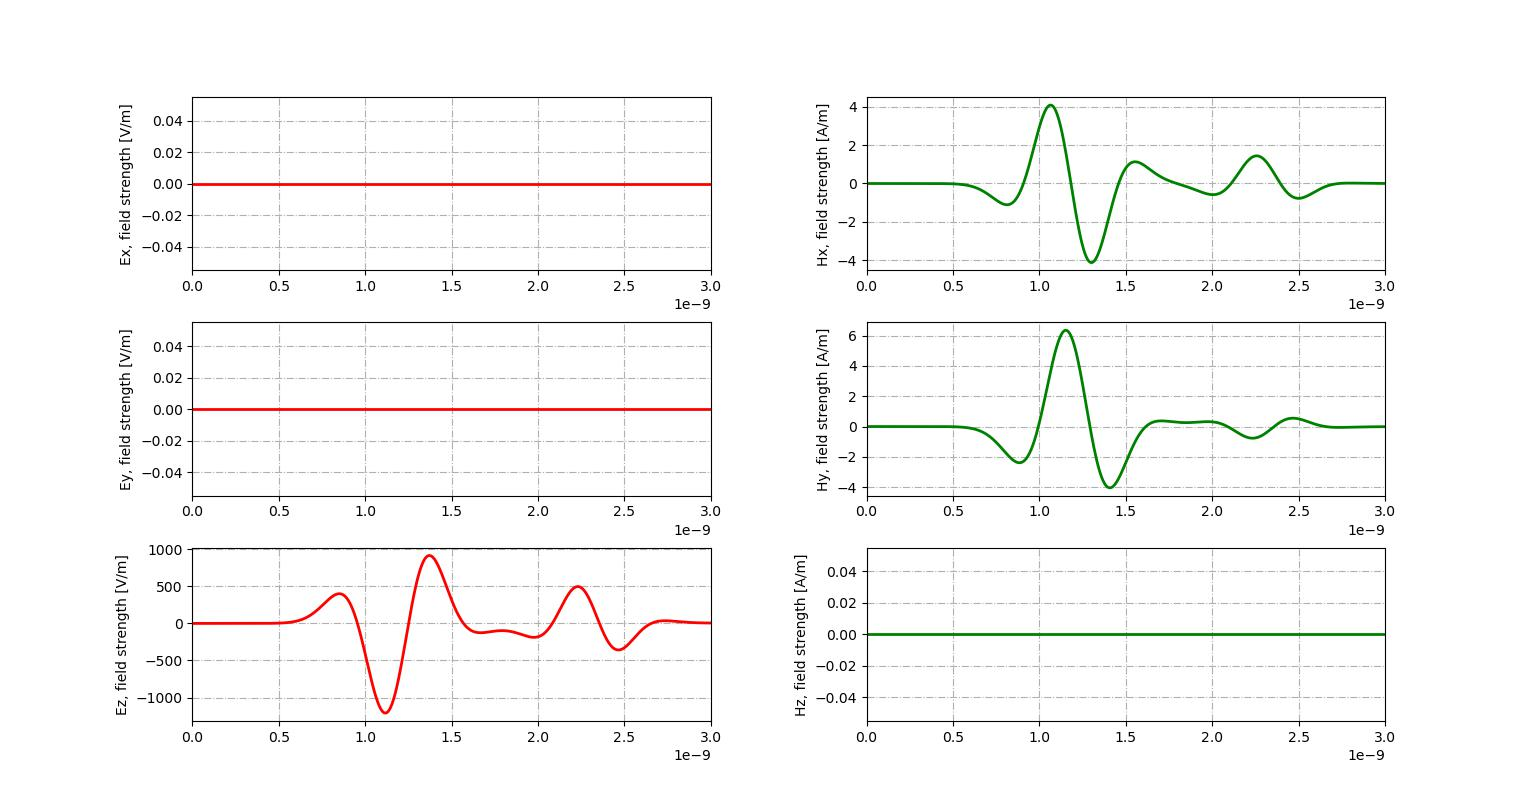
\includegraphics[scale=0.35]{gambar/GPRAscan.jpeg}
  \caption{Contoh A-Scan Sinyal GPR.}
  \label{fig:AscanGPR}
\end{figure}

Bentuk gelombang tunggal atau \emph{A-Scan} didefinisikan sebagai

\begin{equation}
  \label{eq:Ascan}
  F(z)=A( x_{i} , y_{j} , z_{k} )
\end{equation}

di mana rentang k = 1 sampai N, i dan j bilangan konstan \parencite{danielDvd}.
Perlu diperhatikan bahwa waktu dan kedalaman sumbu Z dapat dianggap saling berkaitan dengan kecepatan perambatan.

\subsection{B-Scan}
\label{subsec:bScan}

\emph{B-Scan} merupakan sebuah set dari gelombang radar yang berurutan sepanjang arah tertentu. 
Gambar 2.3 merupakan contoh dari grafik \emph{B-Scan} pada simulasi gprMax. 
Jika \emph{A-Scan} memberikan informasi terkait waktu rambatan antara pengirim dan penerima dalam dimensi spasial, maka sekumpulan gelombang \emph{A-Scan} dapat bekerja baik dalam dimensi temporal maupun spasial.

\begin{figure}[ht]
  \centering
  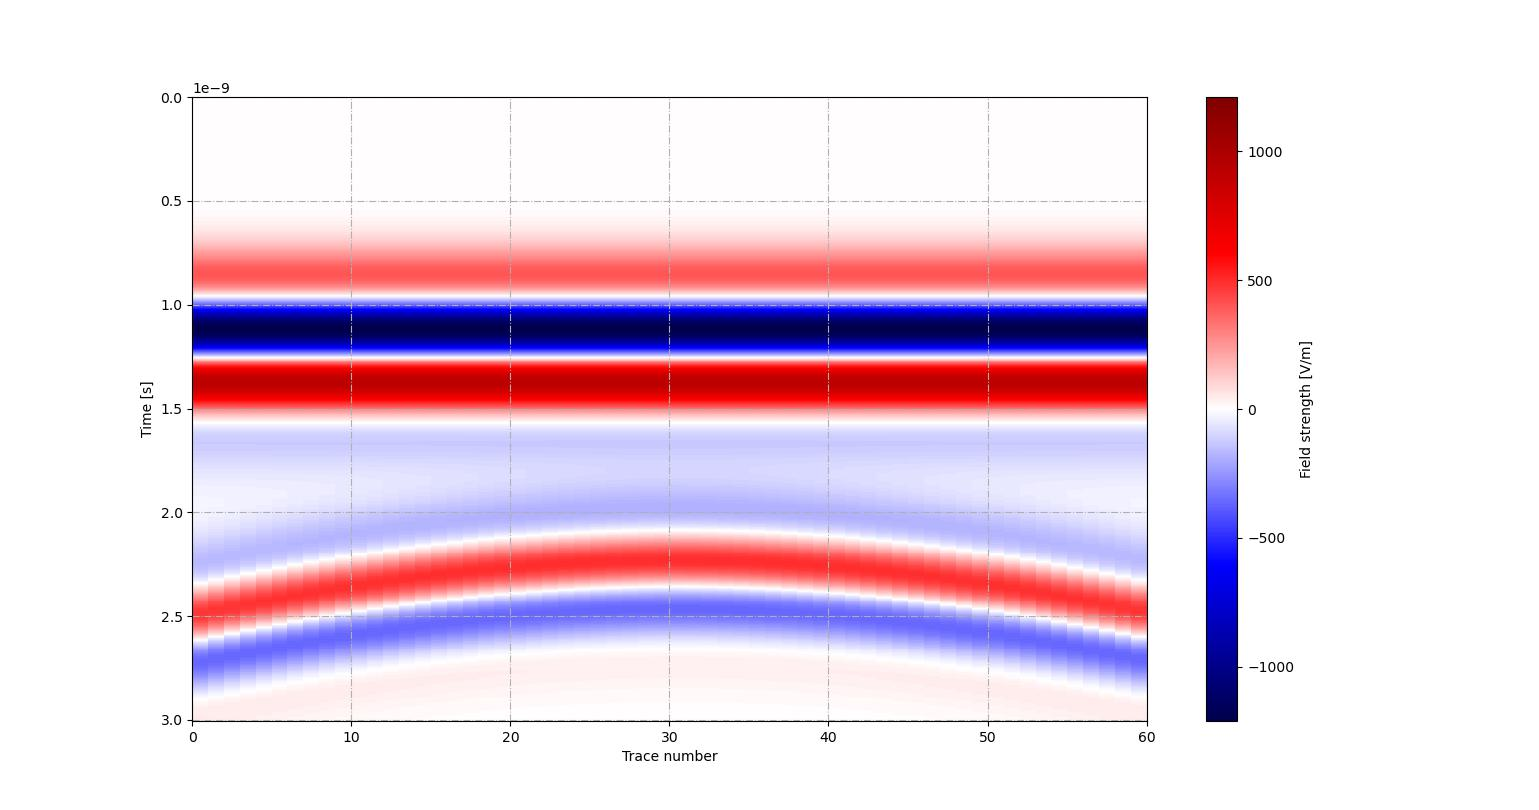
\includegraphics[scale=0.35]{gambar/GPRBscan.jpg}
  \caption{Contoh B-Scan Sinyal GPR.}
  \label{fig:BscanGPR}
\end{figure}

Bentuk gelombang dua dimensi atau B-Scan didefinisikan sebagai

\begin{equation}
  \label{eq:Bscanx}
  F(x,z)=A( x_{i} , y_{j} , z_{k} )
\end{equation}

di mana rentang k = 1 sampai N, i = 1 sampai L, dan j bilangan konstan, atau

\begin{equation}
  \label{eq:Bscany}
  F(y,z)=A( x_{i} , y_{j} , z_{k} )
\end{equation}

di mana rentang k = 1 sampai N, j = 1 sampai M, dan i bilangan konstan \parencite{danielDvd}.

\subsection{Bandwidth}
\label{subsec:bandwidth}

\emph{Bandwidth} merupakan perbedaan antara batas frekuensi tertinggi dengan frekuensi terendah sinyal. 
Pengukuran \emph{Bandwidth} berhubungan langsung dengan resolusi. 
Durasi waktu dari pulsa transmisi berbanding terbalik dengan \emph{bandwidth}. 
Secara matematis, nilai \emph{bandwidth} dan durasi waktu dapat didefinisikan sebagai berikut

\begin{equation}
  \label{eq:BW}
  B \geq  \frac{v}{4 \Delta r} 
\end{equation}

di mana r merupakan panjang resolusi dan v merupakan kecepatan perambatan \parencite{jol2008ground}.

\subsection{Center Frequency}
\label{subsec:centerFrequency}

\emph{Center frequency} merupakan titik tengah dari batas frekuensi atas dan frekuensi bawah. 
\emph{Bandwidth} tidak menentukan frekuensi dari sinyal GPR, namun dapat menentukan batas frekuensi dari \emph{center frequency}.
Semakin rendah frekuensi, semakin besar kemungkinan mendapat sinyal GPR dari media perambatnya.

Sinyal GPR dicirikan oleh rasio bandwidth terhadap \emph{center frequency}

\begin{equation}
  \label{eq:cF}
  R =  \frac{B}{ f_{c} } 
\end{equation}

di mana rasio R diusakan sebesar mungkin \parencite{jol2008ground}. 
Umumnya GPR mencapai rasio R mendekati 1, sehingga \emph{bandwidth} biasa ditafsirkan bernilai sama dengan nilai \emph{center frequency}.

\subsection{Ricker Wavelet}
\label{subsec:rickerWavelet}

Pada GPR, metode pembangkitan data Ricker Wavelet merupakan salah satu metode terbaik dalam membangkitkan data seismik \parencite{rickeronSeismic}. 
Wavelet merupakan satu gelombang pendek, yang diperoleh dari suatu model matematik. 
Wavelet Ricker memungkinkan untuk menggunakan sedikit parameter dalam mendeteksi sinyal seismik.

Ricker wavelet didefinisikan dalam domain waktu sebagai

\begin{equation}
  \label{eq:rickerTimeDomain}
  r(t) =  \big(1 -  \frac{1}{2} (  \omega _{p} ^{2}  t^{2} ) \big)  . exp \big(- \frac{1}{4} ( \omega _{p} ^{2}  t^{2} ) \big) 
\end{equation}

di mana t merupakan waktu dan $\omega_{p}$ merupakan frekuensi sudut puncak.

Spektrum frekuensi dari ricker wavelet dapat didefinisikan sebagai

\begin{equation}
  \label{eq:rickerTimeDomain}
  R( \omega ) =  \big( \frac{2 \omega ^{2}}{  \sqrt{ \pi }  \omega _{p} ^{3}} \big)  . exp \big(- \frac{ \omega ^{2}}{ \omega _{p} ^{2}} \big) 
\end{equation}

\begin{figure}[ht]
  \centering
  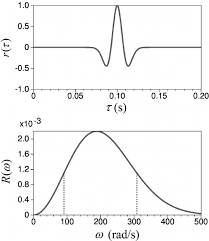
\includegraphics[scale=0.7]{gambar/ricker.jpg}
  \caption{Grafik gelombang ricker beserta spektrum frekuensi \parencite{rickerWavelet}.}
  \label{fig:gelombangRicker}
\end{figure}

Grafik ricker wavelet beserta spektrum frekuensi ditampilkan pada gambar \ref{fig:gelombangRicker}. 
Pada gambar tersebut, digunakan frekuensi sudut puncak $\omega$ = 60$\pi$ rad/s

\section{Neural Networks}
\label{sec:neuralNetworks}

\emph{Neural Network} merupakan salah satu bagian dari \emph{machine learning} yang terinspirasi dari bentuk jaringan neuron pada otak manusia. 
Setiap neuron atau node akan dikumpulkan dalam suatu lapisan (\emph{layers}), yang akan saling berhubungan dan berurutan. 
Pada tingkat paling dasarnya, sebuah jaringan terdiri dari satu node yang mengambil input vektor dikali bobot tertentu, kemudian diubah dengan transformasi non-linear untuk mencapai output yang diharapkan. 
Jaringan juga memiliki lapisan tersembunyi (\emph{hidden layers}), yang beratnya dapat dioptimalkan dalam mencapai output yang diharapkan.

\subsection{Model Generatif}
\label{subsec:modelGeneratif}

Model generatif merupakan bagian dari \emph{Neural Network} yang memungkinkan upaya sintesis dara yang realistis. 
Dasar dari model ini terletak pada \emph{neural network} yang berfungsi secara universal. 
Model ini memungkinkan model, yang awalnya diberi input, mempelajari fitur dari input tersebut, kemudian mampu menghasilkan output yang mirip dengan data input.

\subsection{Generative Adversarial Network}
\label{subsec:generativeAdversarialNetwork}

\emph{Generative Adversarial Network} (GAN) adalah bentuk model generatif, di mana model dibagi menjadi 2 bagian, yaitu bagian generatif (G) dan bagian diskriminator (D). 
Bagian generatif merupakan bagian untuk mensintesis data, sedangkan bagian diskriminator merupakan bagian untuk menentukan apakah data sintesis merupakan data palsu atau asli. 
Model ini seringkali diaplikasikan untuk mereplikasi suatu data, seperti gambar, video, dan audio.

Generator dan Diskriminator akan saling menguntung-rugikan, dengan fungsi V(D,G) direpresentasikan sebagai berikut : 

\begin{equation}
  \label{eq:GAN}
  min_{G} max_{D} V(G,D) =  E_{x \sim p_{data} (x)} \big[ log D(x) \big] + E_{z \sim p_{z} (z)} \big[ log  \big(1-D \big(G(z)\big) \big) \big]
\end{equation}

Dalam mempelajari distribusi generator p pada data x, variabel kebisingan input pz(z) didefinisikan sebelumnya, kemudian pemetaan direpresentasikan ke ruang data sebagai G(z; (teta)g), di mana G adalah fungsi diferensiasi yang direpresentasikan oleh multilayer perceptron dengan parameter (teta)g. 
Multilayer perceptron (MLP) kedua D(x; (teta)d) yang menghasilkan skalar tunggal juga didefinisikan. 
D(x) merepresentasikan kemungkinan bahwa x berasal dari data daripada pg. 
Diskriminator dilatih untuk memaksimalkan kemungkinan menempatkan label yang benar untuk data pelatihan dan sampel dari Generator. 
Generator dan  Diskriminator dilatih secara bersamaan untuk meminimalkan log(1-D(G(z))). \parencite{GAN}

\subsection{Conditional Generative Adversarial Network}
\label{subsec:conditionalGAN}

\emph{Generative Adversarial Network} dapat diperluas ke model bersyarat jika generator dan diskriminator dikondisikan pada beberapa informasi tambahan y. 
Konstanta y bisa berupa segala jenis informasi tambahan, seperti label kelas atau data dari modalitas lain. 
Pengkondisian juga dapat dilakukan dengan memasukkan y ke dalam diskriminator dan generator sebagai lapisan masukan tambahan.

Fungsi dari untung rugi Generator dan Diskriminator V(D,G) untuk \emph{Conditional Generative Adversarial Network} (CGAN) direpresentasikan sebagai berikut :

\begin{equation}
  \label{eq:CGAN}
  min_{G} max_{D} V(G,D) =  E_{x \sim p_{data} (x)} \big[ log D(x|y) \big] + E_{z \sim p_{z} (z)} \big[ log  \big(1-D \big(G(z|y)\big) \big) \big]
\end{equation}

Dalam generator, input kebisingan sebelumnya, pz(z), dan y digabungkan dalam representasi tersembunyi gabungan, dan kerangka pelatihan adversarial memungkinkan fleksibilitas yang cukup besar dalam bagaimana representasi tersembunyi ini disusun. 
Dalam diskriminator x dan y disajikan sebagai input dan ke fungsi diskriminatif (dalam kasus ini diwujudkan kembali oleh MLP). \parencite{CGAN}
